\chapter{PROCEDIMIENTO}

\section{Redes LAN Virtuales}
\begin{caja}[]{
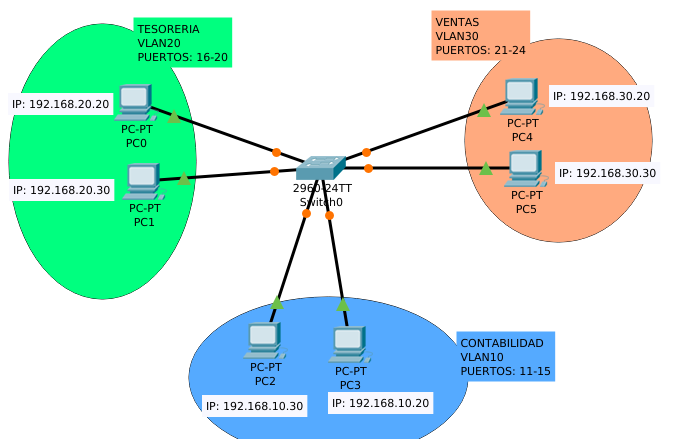
\includegraphics[scale=0.45]{img/exper1.png} 
\end{caja} 

\subsection{EXPERIMENTO 1}

\begin{definicion}[]{
Al simular el env\'io de PDUs o PING, \¿Por qu\'e equipos del
mismo segmento alcanzan su objetivo, en caso contrario no?
}
\end{definicion}

\textbf{mismo segmento} \\
Al hacer la prueba en el mismo segmento o en una misma lan la comunicaci\'on se realiza de manera exitosa. Esto es debido a que ambos host estan en los puertos que corresponden a una misma vlan.\\
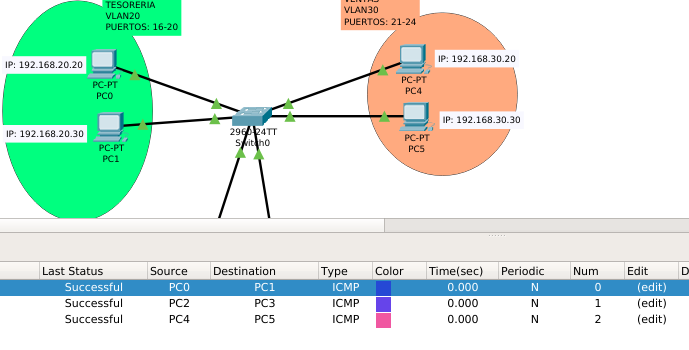
\includegraphics[scale=0.5]{img/mismoseg.png}

\textbf{diferente segmento} \\
Al hacer la prueba en diferentes segmentos la comunicaci\'on no se realiza de manera exitosa. Esto es debido a que no hay comunicacion entre ambos host por que pertenecen a vlans diferentes.\\
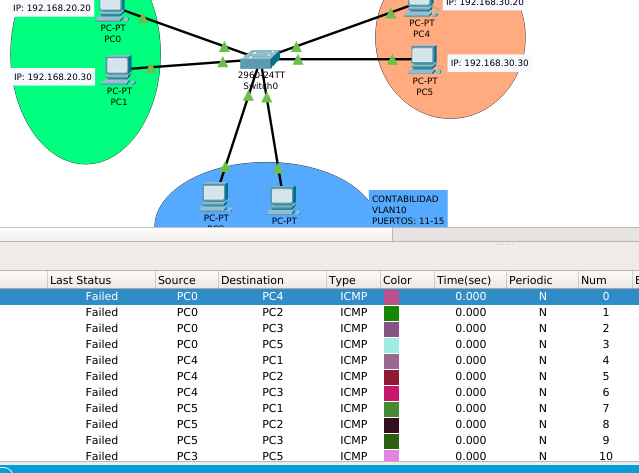
\includegraphics[scale=0.5]{img/segdif.png}  

\subsection{EJERCICIO 01:}
\begin{definicion}[]{
Las VLANs no necesariamente tienen que tener la direcci\'on
de red IP diferente. Implemente dos VLANS en la red
192.20.20.0 que tiene un switch\\
VLAN A equipos con IP 192.20.20.10 y 192.20.20.11, puertos
fast Ethernet 0/10 y fast Ethernet 0/11, respectivamente.\\
VLAN B equipos con IP 192.20.20.12 y 192.20.20.13, puertos
fast Ethernet 0/12 y fast Ethernet 0/13, respectivamente.\\
Equipos fuera de la VLAN con IP 192.20.20.8 y 192.20.20.9,
puertos
fast
Ethernet
0/8
y
fast
Ethernet
0/9,
respectivamente.\\
Simule la red, observe y reflexione sobre porqu\'e s\'i o no,
atribuir\'ia una direcci\'on de red diferente a cada una de
ellas.
}
\end{definicion}

\textbf{construccion}\\
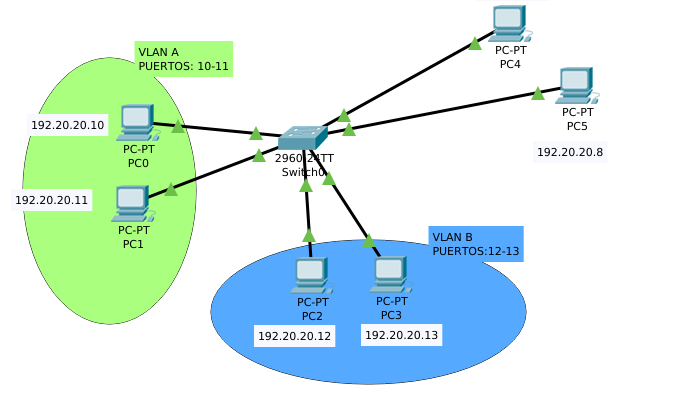
\includegraphics[scale=0.5]{img/ejerc1.png} \\
\textbf{prueba}\\
\textbf{mismo vlan}\\
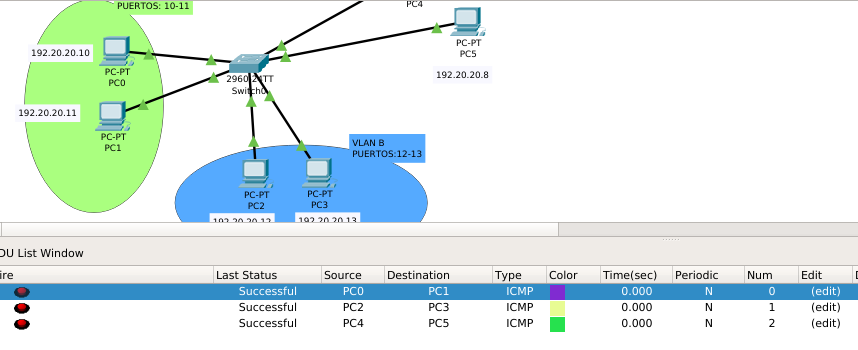
\includegraphics[scale=0.5]{img/succes1.png} 
\\Como se observa la conexion es de manera exitosa.\\
\textbf{diferentes vlan}\\
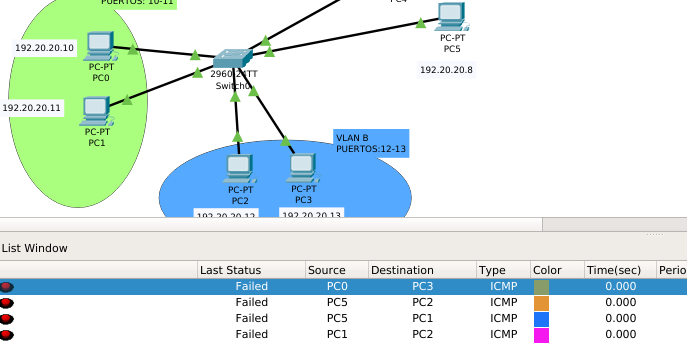
\includegraphics[scale=0.5]{img/failed1.png} \\

\begin{caja}[]{
La razon de asignar las ips a cada vlan es para que podamos segmentar de mejor manera la red. \\
La comunicaci\'on es exitosa ya que estamos usando la configuracion por puertos para asignar cada vlan\\
En el caso de hacer el routing inter vlans necesitaremos asignasr sub redes a las vlans y para ello tenemos que identificar de manera correcta con ips de subredes definidas.
\end{caja} 

\section{Redes LAN Virtuales Extendidas}
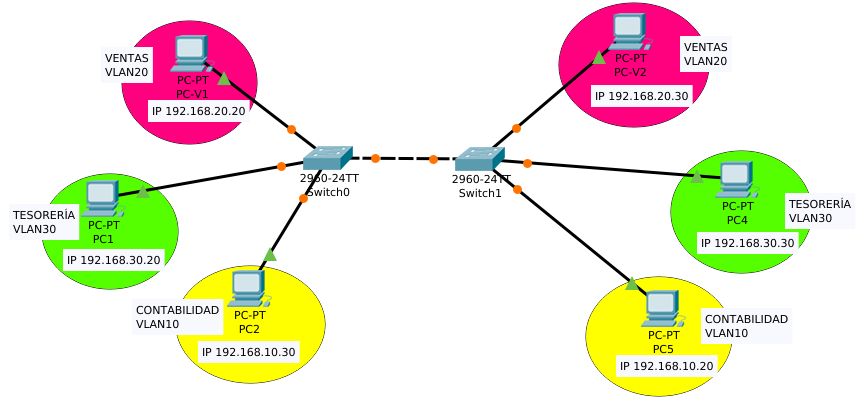
\includegraphics[scale=0.5]{img/exp2.png} 
\subsection{EXPERIMENTO 02}
\begin{definicion}[]{
En el caso de interconectar los switches por el puerto
Gig0/1, es posible asignar el puerto respectivo a una VLAN
(vea Fig. 7) Experimente y observe qu\'e sucede con el acceso
a las otras VLANs?
}
\end{definicion}
Primero probamos cuando asignamos todas las vlans\\
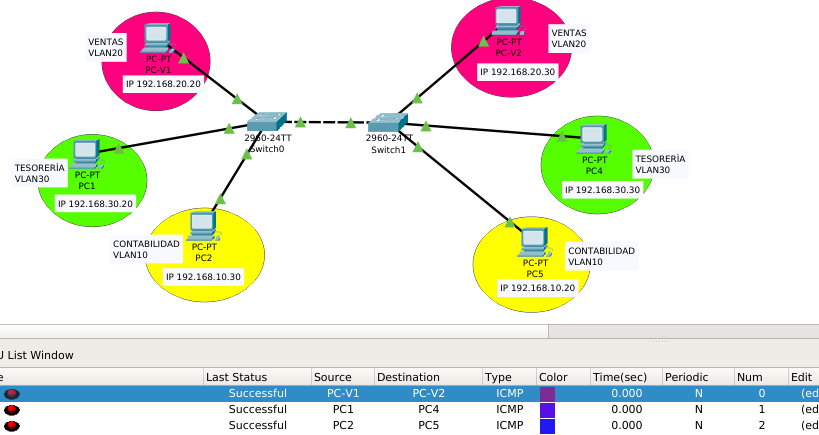
\includegraphics[scale=0.5]{img/primero.png} 
\\ Despues procedemos a asignar solo una vlan.\\
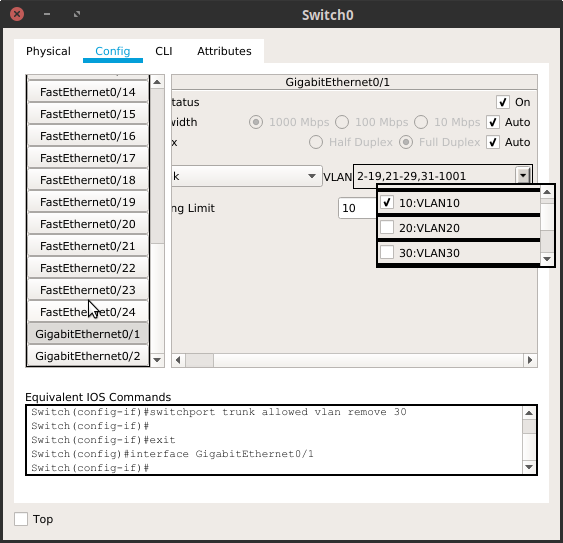
\includegraphics[scale=0.5]{img/vlanconf.png} 
\\probamos\\
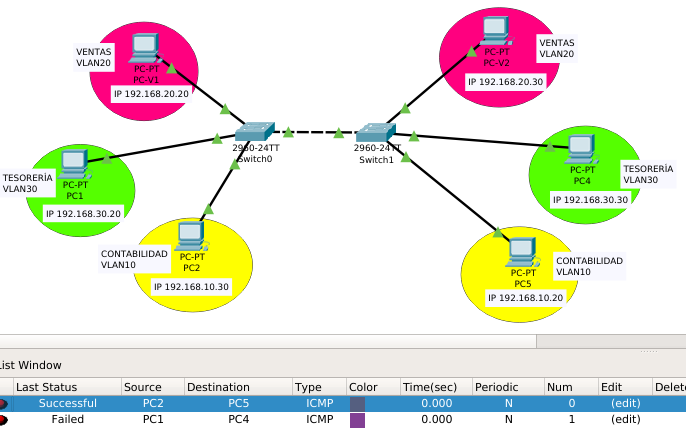
\includegraphics[scale=0.5]{img/sucess10.png} \\
La vlan 10 normal puede comunicarme mientras que las demas vlan no.Esto es debido a que la vlan que cada switch permite que se pueda acceder unicamente es la 10 y no las dem\'as.


\begin{definicion}[]{
Si observa, hay dos tipos de comunicaci\'on: acceso y troncal
(vea Fig. 7). Experimente e infiera cu\'al es la diferencia.
¿En qu\'e modo de conexi\'on deben trabajar los switch para que
funcione la red?
}
\end{definicion}
Sabemos que en el modo troncal se seleccionan las vlan que queremos que tengan permitido comunicarse y todo funciona de manera correcta.\\
En el caso de la conexi\'on de acceso se ve que solo se puede seleccionar una vlan por lo que se intuye que solo permitir\'a acceder a una vlan.
\\
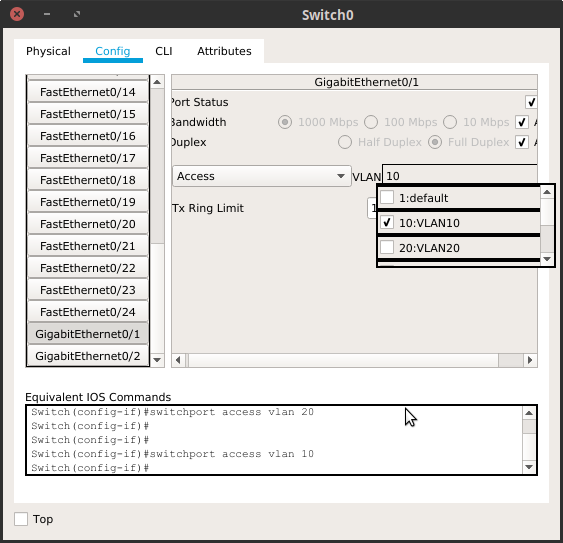
\includegraphics[scale=0.5]{img/access.png} \\
como mencionamos solo se permite el acceso a una sola vlan.\\
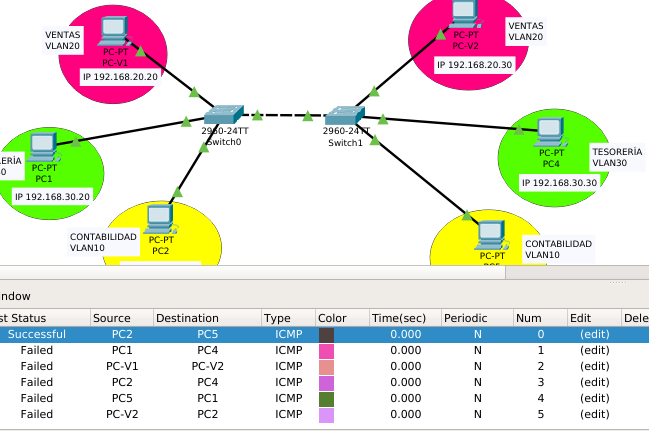
\includegraphics[scale=0.5]{img/dijimos.png} 

\section{Enrutamiento de LAN Virtuales}
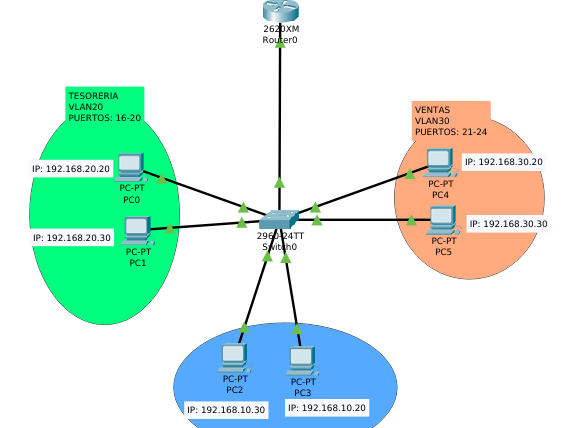
\includegraphics[scale=0.5]{img/enrutam.png} 
\subsection{EXPERIMENTO 03}

\begin{definicion}[]{
Experimente y observe como se realiza el enrutamiento entre
las VLANs
}
\end{definicion}
La maner aen que se realiza esta comunicacion es.\\
Primero se manda al router:\\
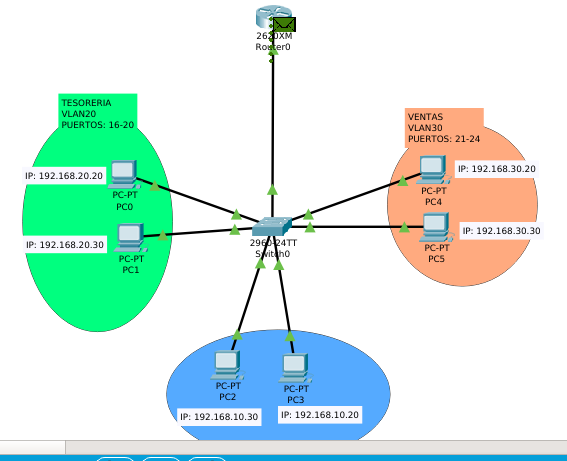
\includegraphics[scale=0.5]{img/1.png} \\
Luego el router lo manda al destino\\
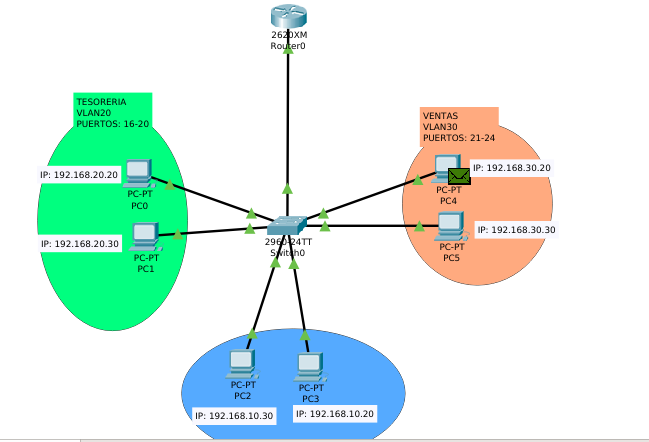
\includegraphics[scale=0.5]{img/2.png} \\
se regresa de nuevo al router\\
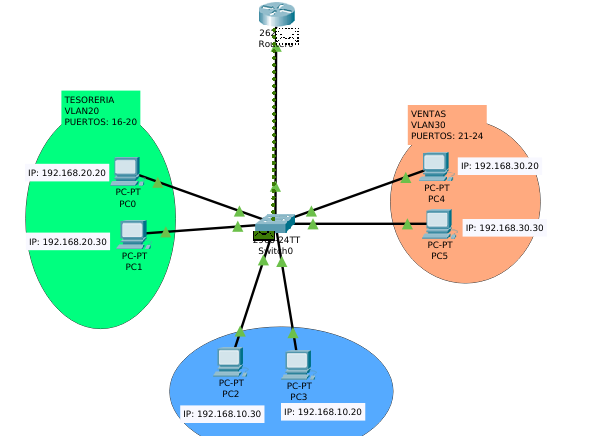
\includegraphics[scale=0.5]{img/3.png} \\
Por ultimo se regresa la respuesta al origen\\
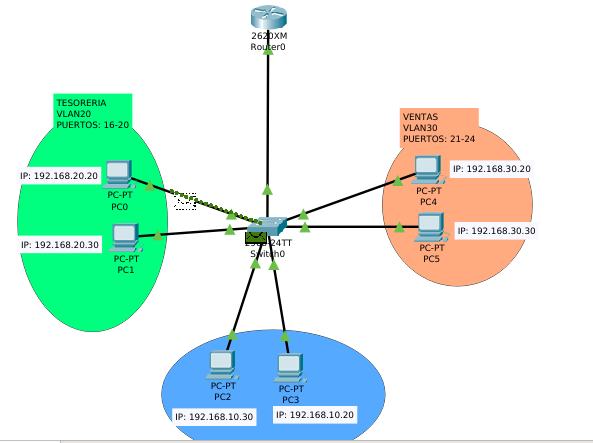
\includegraphics[scale=0.5]{img/4.png} 
\subsection{EJERCICIO 02}
\begin{definicion}[]{
Realice el enrutamiento entre VLANs de la red creada en la
sección 3.2
}
\end{definicion}

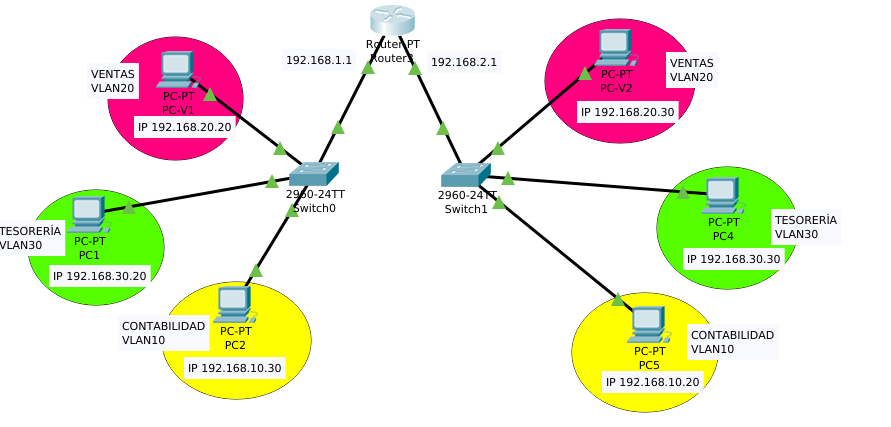
\includegraphics[scale=0.5]{img/routing.png} 
Configuraciones en el router.\\
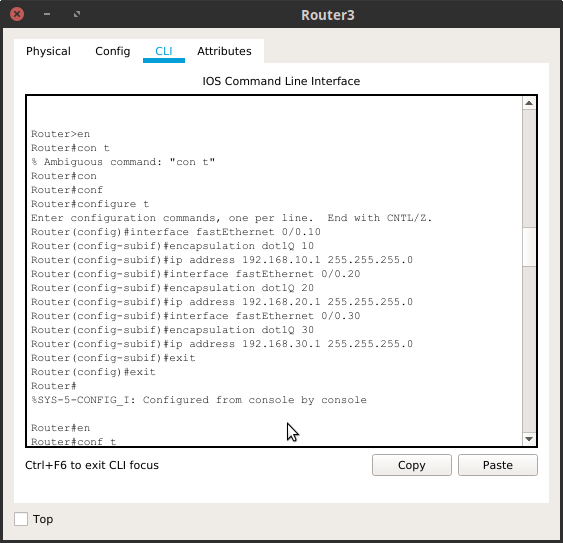
\includegraphics[scale=0.5]{img/1ra.png} \\
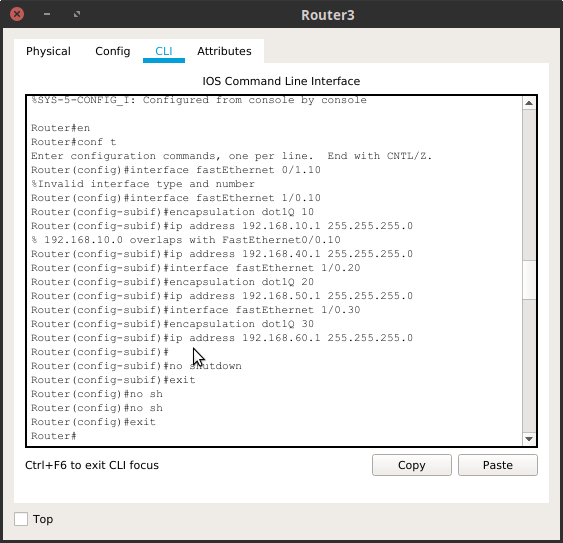
\includegraphics[scale=0.5]{img/2da.png} 
\\ probamos y nos sale:\\
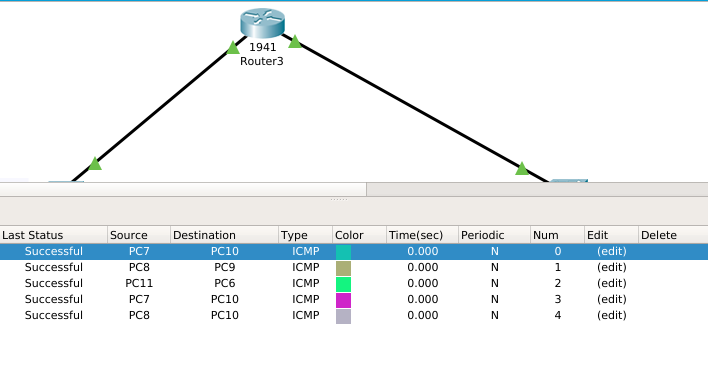
\includegraphics[scale=0.5]{img/salida.png} 

\section{DESAFIO}
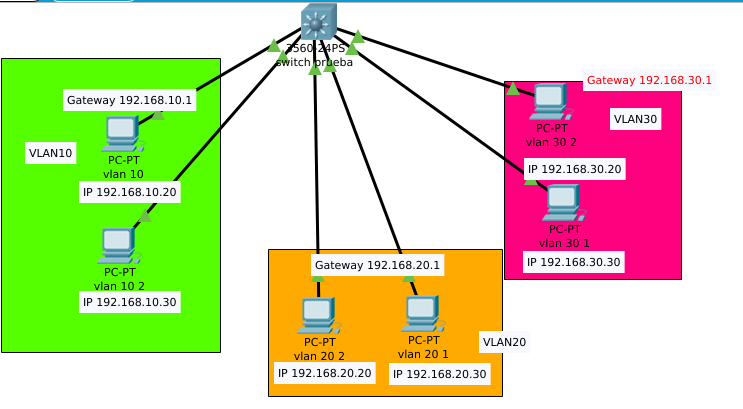
\includegraphics[scale=0.5]{img/DESAFIO.png} 
\\ comprobando que funciona\\
\textbf{VLAN MISMO SEGMENTO}\\
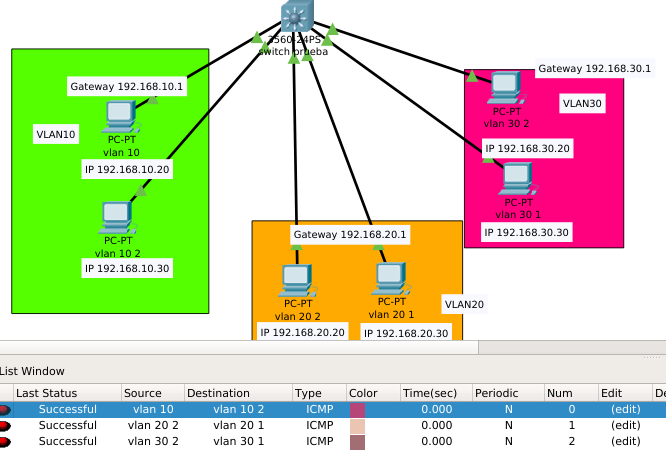
\includegraphics[scale=0.5]{img/11.png} \\
\textbf{VLAN DIFERENTE SEGMENTO}\\
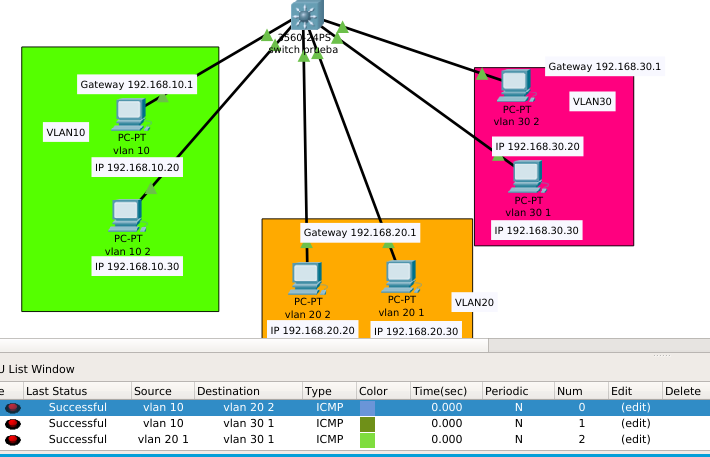
\includegraphics[scale=0.5]{img/00.png} 
